\chapter{Fundamentos}
\label{cap:fundamentos}

Neste capítulo, apresentamos definições fundamentais de teoria dos grafos, teoria da probabilidade e redes bayesianas que o leitor deve conhecer para compreender o trabalho.

Outras definições mais específicas, como as utilizadas para construir o algoritmo para codificar e decodificar \emph{$k$-trees}, estão localizadas nos capítulos subsequentes.

Partimos do pressuposto de que o leitor conhece notações básicas de conjuntos.

\section{Grafos}

Nesta seção apresentamos de forma breve apenas os conceitos de teoria dos grafos necessários para a compreensão deste trabalho. Mais detalhes podem ser encontrados no livro de Bondy e Murty \cite{bondy}, que foi utilizado como referência.

\begin{definition}[grafo]
  Um \textbf{grafo} é um par ordenado $G = (V, E)$. Os elementos de $V$ são chamados de \textbf{vértices} de $G$. Os elementos de $E$ são chamados de \textbf{arestas} de $G$ e consistem em pares (não-ordenados) de vértices distintos\footnote{A rigor, por causa da palavra ``distintos'', essa é a definição do que a literatura costuma chamar de \emph{grafo simples}. Tal definição é utilizada porque neste trabalho não temos interesse em grafos que possuam arestas $(u, v)$ com $u=v$.}. Dados $u, v \in V$, se $(u, v) \in E$ dizemos que $u$ e $v$ são \textbf{adjacentes} em $G$.

  A figura \ref{fig:grafo}(a) mostra como costuma ser representado um grafo. Os vértices são representados pelos círculos e as arestas são representadas pela ligação entre eles. Se $(u, v) \in E$, há uma linha ligando os vértices $u$ e $v$.

  Dado um grafo $G = (V, E)$, o número de arestas que incide num determinado vértice $v \in V$ é chamado de \textbf{grau} do vértice $v$.
\end{definition}

Há diferentes estruturas de dados que podem ser usadas para representar um grafo na memória do computador. Uma das mais comuns, que usamos nas implementações deste trabalho, é a \textbf{lista de adjacência}. Suponha, sem perda de generalidade, que os vértices de um grafo $G$ sejam representados por inteiros de $0$ a $|V|-1$. Então, a representação desse grafo consiste em um vetor de listas {\tt Adj}. A lista {\tt Adj[i]} contém os vértices adjacentes ao vértice de rótulo $i$ (para todo $i \in [0, |V|)$).

\begin{definition}[grafo dirigido]
  Um grafo $G = (V, E)$ é dito \textbf{dirigido} se $E$ consiste em pares \emph{ordenados} de vértices. Se $(a, b) \in E$, dizemos que $a$ aponta para $b$, que há uma aresta de $a$ para $b$ ou que $b$ é filho de $a$.

  A figura \ref{fig:grafo}(b) mostra como costuma ser representado um grafo dirigido. Como o conjunto de arestas consiste em pares ordenados, elas são representadas por setas. Se $(u, v) \in E$, então a seta aponta de $u$ para $v$.
\end{definition}

\begin{definition}[grafo completo]
  Um grafo $G = (V, E)$ é dito \textbf{completo} se $(u, v) \in E$ para todo $u, v \in V, u \neq v$. Um grafo completo com $n$ vértices é geralmente denotado $K_n$.

  Na figura \ref{fig:grafo}(c), a representação de um grafo completo com $4$ vértices.
\end{definition}

\begin{figure}
  \begin{minipage}{0.3333\textwidth}
    \centering
    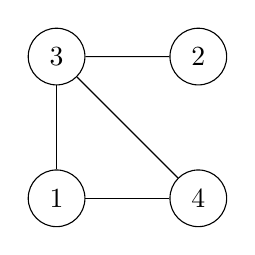
\begin{tikzpicture}
        [scale=.6,auto=left,every node/.style={draw, circle, inner sep = 0pt, minimum width = 0.72cm}]
      \node (n1) at (1,1) {1};
      \node (n2) at (4,4) {2};
      \node (n3) at (1,4) {3};
      \node (n4) at (4,1) {4};

      \foreach \from/\to in {n1/n3, n1/n4, n2/n3, n3/n4}
        \draw (\from) edge (\to);
    \end{tikzpicture}

    (a)
  \end{minipage}\begin{minipage}{0.3333\textwidth}
    \centering
    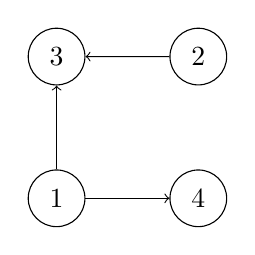
\begin{tikzpicture}
        [scale=.6,auto=left,every node/.style={draw, circle, inner sep = 0pt, minimum width = 0.72cm}]
      \node (n1) at (1,1) {1};
      \node (n2) at (4,4) {2};
      \node (n3) at (1,4) {3};
      \node (n4) at (4,1) {4};

      \foreach \from/\to in {n1/n3, n1/n4, n2/n3}
        \draw (\from) edge[->] (\to);
    \end{tikzpicture}

    (b)
  \end{minipage}\begin{minipage}{0.3333\textwidth}
    \centering
    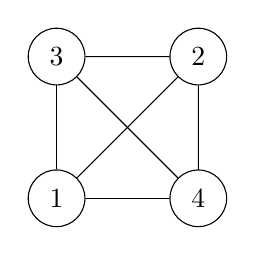
\begin{tikzpicture}
        [scale=.6,auto=left,every node/.style={draw, circle, inner sep = 0pt, minimum width = 0.72cm}]
      \node (n1) at (1,1) {1};
      \node (n2) at (4,4) {2};
      \node (n3) at (1,4) {3};
      \node (n4) at (4,1) {4};

      \foreach \from/\to in {n1/n2, n1/n3, n1/n4, n2/n3, n2/n4, n3/n4}
        \draw (\from) edge (\to);
    \end{tikzpicture}

    (c)
  \end{minipage}

  \caption{
    \textbf{(a)} Representação do grafo $G = (V_G, E_G)$ com $V_G = \{1, 2, 3, 4\}$ e $E_G = \{(1, 3), (1, 4), (2, 3), (3, 4)\}$.
    \textbf{(b)} Representação do grafo dirigido $D = (V_D, E_D)$ com $V_D = \{1, 2, 3, 4\}$ e $E_D = \{(1, 3), (1, 4), (2, 3)\}$.
    \textbf{(c)} Representação do $K_4$, o grafo completo com $4$ vértices.
  }
  \label{fig:grafo}
\end{figure}

\begin{definition}[subgrafo]
  Um grafo $F = (V_F, E_F)$ é chamado de \textbf{subgrafo} de $G = (V_G, E_G)$ se $V_F \subseteq V_G$ e $E_F \subseteq E_G$.
\end{definition}

\begin{definition}[subgrafo induzido]
  Dado um grafo $G = (V, E)$ e um subconjunto $V'$ de $V$, o subgrafo de $G$ \textbf{induzido} por $V'$, $G' = (V', E')$, é o grafo formado pelos vértices $V' \subseteq V$ e arestas que só contém elementos de $V'$, ou seja, $E' = \{(u, v) \in E \ | \  u, v \in V'\}$.
\end{definition}

\begin{definition}[$k$-clique]
  Seja $G = (V, E)$ um grafo. Um \textbf{$k$-clique} (também chamado de \textbf{clique de tamanho $k$}) é um subconjunto dos vértices, $C \subseteq V$, tal que $(u, v) \in E \ \forall \ u, v \in C, u \neq v$ (ou seja, tal que o subgrafo induzido por $C$ é completo).
\end{definition}

\begin{definition}[caminho]
  Dado um grafo $G = (V, E)$, um \textbf{caminho} em $G$ é um subgrafo de $G$ cujos vértices podem ser arranjados numa sequência linear de forma que dois vértices são adjacentes se eles são consecutivos na sequência e não-adjacentes caso contrário. Se $u, v \in V$ pertencem a um caminho $P$, dizemos que eles estão conectados pelo caminho $P$.
\end{definition}

\begin{definition}[distância]
  Dado um grafo $G = (V, E)$ e dois vértices $(u, v) \in V$, a \textbf{distância} entre $u$ e $v$ é o número de arestas num menor caminho que os conecte.
\end{definition}

\begin{definition}[ciclo]
  Dado um grafo $G = (V, E)$, um \textbf{ciclo} em $G$ é um caminho formado por vértices $x_1, \cdots, x_k \in V$ onde $x_1 = x_k$.
\end{definition}

\begin{definition}[DAG]
  Um grafo $G = (V, E)$ é chamado de \textbf{DAG} (do inglês \emph{directed acyclic graph}: grafo dirigido acíclico) se ele é dirigido e não possui ciclos.
\end{definition}

Dizemos que um ciclo tem uma \textbf{corda} se dois vértices no ciclo são conectados por uma aresta que não está no ciclo. Um \textbf{grafo cordal} é um grafo no qual todos os ciclos com pelo menos $4$ vértices têm uma corda. Qualquer grafo pode ser transformado num grafo cordal adicionando-se arestas num processo chamado de \textbf{cordalização}.

O \textbf{grafo moral} de um DAG $G = (V, E)$ é um grafo não-dirigido obtido conectando-se todo par de vértices com um filho em comum e retirando a direção das arestas.

\begin{definition}[treewidth]
  \cite{maua} Dado um grafo $G = (V, E)$, seu \textbf{\emph{treewidth}} é um inteiro definido da seguinte forma:

  \begin{itemize}
    \item Se $G$ é um grafo cordal, então seu \emph{treewidth} é o tamanho do seu maior clique menos 1.
    \item Se $G$ é um grafo não-dirigido arbitrário, então seu \emph{treewidth} é o mínimo entre os \emph{treewidth} de todas as suas cordalizações.
    \item Se $G$ é um DAG, então seu \emph{treewidth} é o \emph{treewidth} do seu grafo moral.
  \end{itemize}
\end{definition}

\begin{definition}[árvore]
  Dado um grafo $G = (V, E)$, dizemos que ele é uma \textbf{árvore} se cada dois vértices $u, v \in V$ são conectados por exatamente um caminho.
\end{definition}

Dada uma árvore $T = (V, E)$, os vértices em $V$ que tem grau $1$ são chamados de \textbf{folhas}.

Dada uma árvore $T = (V, E)$, às vezes é conveniente destacar um vértice $r \in V$ e chamá-lo de \textbf{raiz} da árvore $T$. Chamamos o par formado pela árvore $T$ e pela raiz $r \in V$ de \textbf{árvore enraizada}.

\subsection{\emph{$k$-trees}}

\begin{definition}[\emph{$k$-tree}]
  \label{def:ktree}
  \cite{harary} Uma \textbf{\emph{$k$-tree}} é definida da seguinte forma recursiva:

  \begin{enumerate}
    \item Um grafo completo com $k$ vértices é uma \emph{$k$-tree}.
    \item Se $T_k' = (V, E)$ é uma \emph{$k$-tree}, $K \subseteq V$ é um $k$-clique e $v \not \in V$, então $T_k = (V \cup \{v\}, E \cup \{(v,x) \ | \  x \in K\})$ é uma \emph{$k$-tree}.
  \end{enumerate}

  Na figura \ref{fig:ktree}(a), um exemplo de \emph{$k$-tree} com $k = 1$ (ou seja, uma árvore comum) e $n = 4$ vértices rotulados com inteiros em $[1, 4]$; na figura \ref{fig:ktree}(b), um exemplo de \emph{$k$-tree} com $k = 2$ e $n = 5$ vértices rotulados com inteiros em $[1, 5]$; na figura \ref{fig:ktree}(c), um exemplo de \emph{$k$-tree} com $k = 3$ e $n = 5$ vértices rotulados em $[1, 5]$.

  \begin{figure}
    \begin{minipage}{0.3333\textwidth}
      \centering
      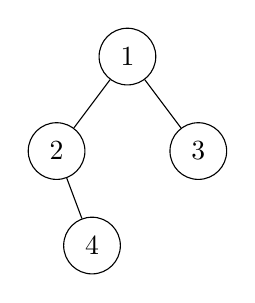
\begin{tikzpicture}
          [scale=.6,auto=left,every node/.style={draw, circle, inner sep = 0pt, minimum width = 0.72cm}]
        \node (n1) at (3,8) {1};
        \node (n2) at (1.5,6) {2};
        \node (n3) at (4.5,6) {3};
        \node (n4) at (2.25,4) {4};

        \foreach \from/\to in {n1/n2, n1/n3, n2/n4}
          \draw (\from) edge (\to);
      \end{tikzpicture}

      (a)
    \end{minipage}\begin{minipage}{0.3333\textwidth}
      \centering
      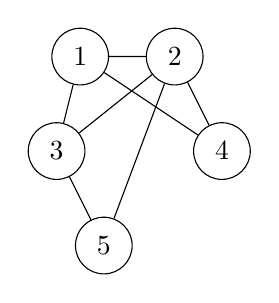
\begin{tikzpicture}
          [scale=.6,auto=left,every node/.style={draw, circle, inner sep = 0pt, minimum width = 0.72cm}]
        \node (n1) at (3,8) {1};
        \node (n2) at (5,8) {2};
        \node (n3) at (2.5,6) {3};
        \node (n4) at (6,6) {4};
        \node (n5) at (3.5,4) {5};

        \foreach \from/\to in {n1/n2, n3/n1, n3/n2, n4/n1, n4/n2, n5/n3, n5/n2}
          \draw (\from) edge (\to);
      \end{tikzpicture}

      (b)
    \end{minipage}\begin{minipage}{0.3333\textwidth}
      \centering
      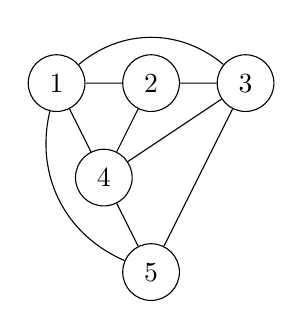
\begin{tikzpicture}
          [scale=.6,auto=left,every node/.style={draw, circle, inner sep = 0pt, minimum width = 0.72cm}]
        \node (n1) at (3,8) {1};
        \node (n2) at (5,8) {2};
        \node (n3) at (7,8) {3};
        \node (n4) at (4,6) {4};
        \node (n5) at (5,4) {5};

        \foreach \from/\to in {n1/n2, n2/n3, n1/n4, n2/n4, n3/n4, n4/n5, n3/n5}
          \draw (\from) edge (\to);

        \draw (n1) edge [bend left=40] (n3);
        \draw (n1) edge [bend right=40] (n5);
      \end{tikzpicture}

      (c)
    \end{minipage}

    \caption{
      \textbf{(a)} Uma \emph{$1$-tree} (ou seja, uma árvore comum) com $4$ vértices.
      \textbf{(b)} Uma \emph{$2$-tree} com $5$ vértices.
      \textbf{(c)} Uma \emph{$3$-tree} com $5$ vértices.
    }
    \label{fig:ktree}
  \end{figure}
\end{definition}

\begin{definition}[\emph{$k$-tree} enraizada]
  \cite{caminiti} Uma \textbf{\emph{$k$-tree} enraizada} é uma \emph{$k$-tree} com um $k$-clique destacado $R = \{r_1, r_2, \cdots, r_k\}$ que é chamado de \emph{raiz} da \emph{$k$-tree} enraizada.

  Na figura \ref{fig:rootedktree}(a), um exemplo de uma \emph{$k$-tree} com $k = 3$ e $n = 11$ vértices rotulados com inteiros em $[1, 11]$. Na figura \ref{fig:rootedktree}(b), a mesma \emph{$k$-tree}, dessa vez enraizada no $3$-clique $R = \{2, 3, 9\}$.

  \begin{figure}
    \begin{minipage}{0.5\textwidth}
      \centering
      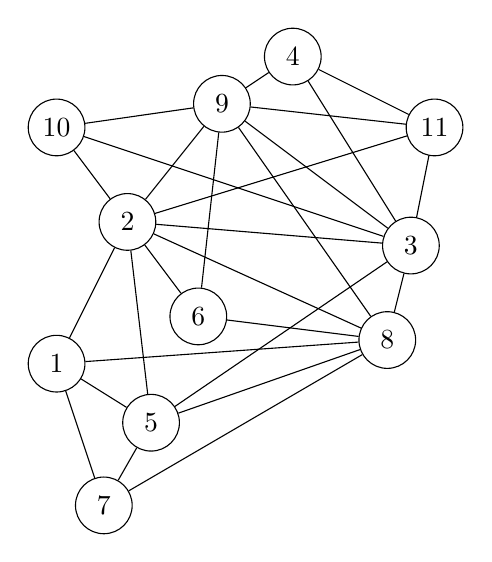
\begin{tikzpicture}
          [scale=.6,auto=left,every node/.style={draw, circle, inner sep = 0pt, minimum width = 0.72cm}]
        \node (n10) at (1,9) {10};
        \node (n2) at (2.5,7) {2};
        \node (n1) at (1,4) {1};
        \node (n5) at (3,2.75) {5};
        \node (n7) at (2,1) {7};
        \node (n9) at (4.5,9.5) {9};
        \node (n6) at (4,5) {6};
        \node (n4) at (6,10.5) {4};
        \node (n3) at (8.5,6.5) {3};
        \node (n8) at (8,4.5) {8};
        \node (n11) at (9,9) {11};

        \foreach \from/\to in {n1/n2, n1/n5, n1/n7, n1/n8, n2/n3, n2/n5, n2/n6, n2/n8, n2/n9, n2/n10, n2/n11, n3/n4, n3/n5, n3/n8, n3/n9, n3/n10, n3/n11, n4/n9, n4/n11, n5/n7, n5/n8, n6/n8, n6/n9, n7/n8, n8/n9, n9/n10, n9/n11}
          \draw (\from) edge (\to);
      \end{tikzpicture}

      (a)
    \end{minipage}\begin{minipage}{0.5\textwidth}
      \centering
      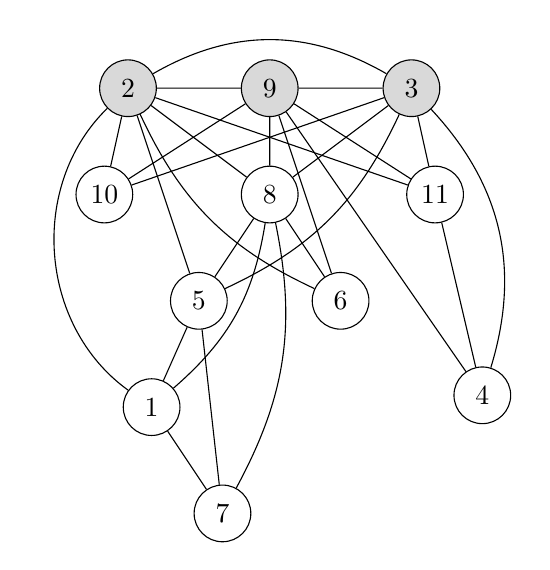
\begin{tikzpicture}
          [scale=.6,auto=left,every node/.style={draw, circle, inner sep = 0pt, minimum width = 0.72cm}]
        \node (n10) at (1,8.25) {10};
        \node[fill=gray!30] (n2) at (1.5,10.5) {2};
        \node (n1) at (2,3.75) {1};
        \node (n5) at (3,6) {5};
        \node (n7) at (3.5,1.5) {7};
        \node[fill=gray!30] (n9) at (4.5,10.5) {9};
        \node (n6) at (6,6) {6};
        \node (n4) at (9,4) {4};
        \node[fill=gray!30] (n3) at (7.5,10.5) {3};
        \node (n8) at (4.5,8.25) {8};
        \node (n11) at (8,8.25) {11};

        \foreach \from/\to in {n1/n5, n1/n7, n2/n5, n2/n8, n2/n9, n2/n10, n2/n11, n3/n8, n3/n9, n3/n10, n3/n11, n4/n9, n4/n11, n5/n7, n5/n8, n6/n8, n6/n9, n8/n9, n9/n10, n9/n11}
          \draw (\from) edge (\to);

        \draw (n1) edge [bend right=20] (n8);
        \draw (n1) edge [bend left=50] (n2);
        \draw (n2) edge [bend left] (n3);
        \draw (n2) edge [bend right=20] (n6);
        \draw (n3) edge [bend left] (n4);
        \draw (n3) edge [bend left=20] (n5);
        \draw (n7) edge [bend right=20] (n8);
      \end{tikzpicture}

      (b)
    \end{minipage}

    \caption{
      \textbf{(a)} Uma \emph{$3$-tree} $T_3$ com 11 vértices.
      \textbf{(b)} A mesma \emph{$3$-tree} ($T_3$) enraizada no $3$-clique $\{2, 3, 9\}$.
    }
    \label{fig:rootedktree}
  \end{figure}
\end{definition}

\begin{definition}[\emph{partial $k$-tree}]
  \cite{bodlaender} Um subgrafo de uma \emph{$k$-tree} é chamado de \textbf{\emph{partial $k$-tree}}. Um grafo é uma \emph{partial $k$-tree} se e só se ele tem \emph{treewidth} menor ou igual a $k$.
\end{definition}

\section{Probabilidade}

Nesta seção apresentamos de forma sintética alguns conceitos de teoria da probabilidade necessários para a compreensão deste trabalho. Mais detalhes podem ser encontrados no livro de Koller e Friedman \cite{koller}, que foi utilizado como referência.

Um \textbf{experimento aleatório} é um fenômeno que possui resultado imprevisível. Por exemplo, o lançamento de um dado de seis faces é um experimento aleatório.

O \textbf{espaço amostral} de um experimento aleatório, geralmente denotado $\Omega$, é o conjunto de todos os resultados possíveis do experimento. Por exemplo, o espaço amostral do lançamento de um dado de seis faces é $\{1, 2, 3, 4, 5, 6\}$.

\textbf{Eventos} são subconjuntos de um espaço amostral para os quais pretendemos atribuir probabilidades. Por exemplo, no lançamento de um dado de seis faces o evento $\{6\}$ corresponde ao caso em que o lançamento resulta em $6$ e o evento $\{1, 2\}$ corresponde ao caso em que o lançamento resulta em $1$ ou $2$.

A teoria da probabilidade requer que o espaço dos eventos $S \subseteq \Omega$ satisfaça três propriedades:

\begin{itemize}
  \item Deve conter o \textbf{evento vazio} $\emptyset$ e o \textbf{evento trivial} $\Omega$.
  \item Se $\alpha, \beta \in S$, então $\alpha \cup \beta \in S$.
  \item Se $\alpha \in S$, então $\Omega \setminus \alpha \in S$.
\end{itemize}

O requisito de que o espaço dos eventos é fechado sob a união e o complemento implica que ele também seja fechado sob outras operações booleanas como interseção e diferença.

\begin{definition}[distribuição de probabilidade]
  Seja $\Omega$ um espaço amostral e $S$ um espaço de eventos. Uma \textbf{distribuição de probabilidade} $P$ sobre $(\Omega, S)$ é um mapeamento dos eventos em $S$ para valores reais que satisfaz as seguintes condições:

  \begin{itemize}
    \item Probabilidades são não-negativas, ou seja, $P(\alpha) \geq 0$ para todo $\alpha \in S$.
    \item O evento trivial tem a maior probabilidade possível, ou seja, $P(\Omega) = 1$.
    \item A probabilidade de que um de dois eventos disjuntos ocorra é a soma das probabilidades de cada evento, ou seja, se $\alpha, \beta \in S$ e $\alpha \cup \beta = \emptyset$, então $P(\alpha \cup \beta) = P(\alpha) + P(\beta)$.
  \end{itemize}

  Essas condições implicam em outras. Em particular, vale destacar que $P(\emptyset) = 0$ e $P(\alpha \cup \beta) = P(\alpha) + P(\beta) - P(\alpha \cap \beta)$.
\end{definition}

\begin{definition}[probabilidade condicional]
  Seja $P$ uma distribuição de probabilidade sobre $(\Omega, S)$ e sejam $\alpha, \beta \in S$. A \textbf{probabilidade condicional} de $\beta$ dado $\alpha$, $P(\beta | \alpha)$, é definida como:

  $$P(\beta | \alpha) = \frac{P(\alpha \cap \beta)}{P(\alpha)}$$
\end{definition}

Duas consequências da definição da probabilidade condicional são as fórmulas que chamamos de \textbf{regra da cadeia} e \textbf{regra de Bayes}:

\begin{description}
  \item[Regra da Cadeia.] Se $\alpha_1, \cdots, \alpha_k \in S$, então

    $$P(\alpha_1 \cap \cdots \alpha_k) = P(\alpha_1) P(\alpha_2 | \alpha_1) \cdots P(\alpha_k | \alpha_1 \cap \cdots \cap \alpha_{k-1})$$

  \item[Regra de Bayes.] Se $\alpha, \beta \in S$, então

    $$P(\alpha | \beta) = \frac{P(\beta | \alpha) P(\alpha)}{P(\beta)}$$
\end{description}

\vspace{2em}

A continuar (variável aleatória, probabilidade conjunta, independência).
% TODO: variável aleatória
% TODO: probabilidade conjunta
% TODO: independência

\subsection{Redes bayesianas}

Redes bayesianas são modelos probabilísticos gráficos que representam distribuições de probabilidade conjunta e são usados para raciocinar em situações com incerteza. Formalmente:

\begin{definition}[rede bayesiana]
  \cite{maua}
  Seja $N = \{ 1, \cdots, n \}$ e seja $X = \{X_i : i \in N\}$ um conjunto de variáveis aleatórias $X_i$ tomando valores em conjuntos finitos $\mathcal{X}_i$. Uma \textbf{rede bayesiana} é uma tripla $(X, G, \pi)$, onde $G = (V, E)$ é um DAG (que chamamos de \textbf{estrutura} da rede bayesiana) cujos vértices correspondem a variáveis em $X$ e $\pi = \{\pi_i(x_i, x_{\pi_i})\}$ é um conjunto de parâmetros numéricos especificando valores de probabilidade condicional $\pi_i(x_i, x_{\pi_i}) = P(x_i | x_{\pi_i})$ para todo vértice $i \in V$, valor $x_i \in X_i$ e atribuição $x_{\pi_i}$ para os pais $\pi_i$ de $X_i$ (em $G$).
\end{definition}

Redes bayesianas são geralmente usadas para fazer inferências como computar a probabilidade de alguma variável depois que alguma evidência é observada. Por exepmlo, uma rede bayesiana pode representar as relações de probabilidade entre doenças e sintomas. Observados alguns sintomas, a rede pode ser usada para computar a probabilidade da presença das doenças.

No capítulo \ref{cap:aprendizado}, discutimos o problema de aprender estruturas de redes bayesianas a partir de dados.
